\chapter{Annotate French Clinical Data Using Large Language Model Predictions}

In clinical and other specialized domains, data are scarce due to their confidential nature. This lack of data is a major problem when fine-tuning language models.
Nevertheless, very large language models (LLMs) are promising for the medical domain but cannot be used directly in healthcare facilities due to data confidentiality issues. We explore an approach of annotating training data with LLMs to train smaller models more adapted to our problem. 
We show that this method yields promising results for information extraction tasks.

\section{Introduction}
Clinical notes contain the interactions between the patient and healthcare staff. Professionals record their impressions, observations, and various medical procedures performed. Despite the computerization of clinical documents, notes should remain fairly expressive and in a free format to save time for healthcare personnel and allow for the description of unusual situations \citep{Rosenbloom2011DataDocumentation}. Moreover, a large amount of crucial information is exclusively contained in clinical notes. According to a study by \citet{Escudie2017ADisease}, approximately 80\% of patient phenotypes (a set of observable biological and physical characteristics that can characterize a disease) are present only in free text. These documents are difficult to use without advanced methods such as deep learning in NLP. The use of such methods requires the collection and annotation of a significant amount of medical data. However, \citet{Fries2022DatasetModeling} proposes the term "dataset debt," which highlights the fact that learning data in the biomedical field is poorly accessible, poorly documented, and opaque as to its reusability in a commercial or a hospital context. According to the article, only 13\% of the 167 analyzed datasets are accessible and downloadable, 22\% use a standard structured format, and 40\% are in the public domain.

In recent years, large language models (LLMs) have proved their ability to perform a wide range of tasks with high accuracy in a zero-shot or a few-shots contexts.
This trend holds great potential for clinical NLP, as preliminary results show promise for information extraction tasks \citep{Agrawal2022LargeExtractors}. 
However, the clinical domain presents unique challenges due to the confidential and linguistically specific nature of its data, which can make collection and annotation time-consuming and expensive.
Using LLMs for efficient information extraction without training data could be attractive, but it raises confidentiality concerns.
The model deployment should be controllable, and the model's prediction should evolve to fit a specific and changing annotation guideline.
Most LLMs are not freely available \citep{Scao2022BLOOM:Model,Ouyang2022TrainingFeedback,Thoppilan2022LaMDA:Applications}, to the best of our knowledge, only BLOOM is open-source and deployable in a custom infrastructure. The computing resources to use these models remains challenging for healthcare establishments.

One approach to address these issues is to distil LLMs into a smaller model via weak supervision. 
Weak supervision has recently gained community attention because it alleviates the annotation task. This technique refers to annotating datasets using rule-based, heuristic, dictionary extraction or more advanced methods and then training the smaller model on this dataset.
In the same way, knowledge distillation aims to transfer knowledge from a master model to a student model. It has often been used to compress large-scale models to improve memory footprint and the inference speed \citep{Li2021DynamicModels}. 
Moreover, student models trained through knowledge distillation can be more easily monitored and versioned. Hosting them increases the healthcare centre's sovereignty, and they become more compliant with existing privacy policies, as input data or predictions don't leave the building.

\section{Motivation and Contributions}
Our works study the use of LLMs in the knowledge distillation technique via weak supervision techniques in the French Clinical domain, especially in clinical entity extraction. We extend the \citet{Agrawal2022LargeExtractors} study in the sense that we propose an in-depth study of the use of InstructGPT-3 to annotate a training dataset. Our work mainly aims to compare the annotation quality using weak supervision tasks on a smaller model (Figure \ref{fig:healthnlp_motiv}). Finally, we propose to combine annotations provided by InstructGPT-3 and the dictionary extraction method.

This takes form in these contributions:
\begin{itemize}
    \item We show that InstructGPT-3 distillation (Figure \ref{fig:healthnlp_motiv} middle) is a competitive technique compared to classic weak-supervision techniques in the french clinical domain;
    \item We propose a weak supervision approach (Figure \ref{fig:healthnlp_motiv} bottom) that combines annotations from dictionary extraction and LLM predictions to create a training dataset which outperforms annotations from InstructGPT-3 predictions alone.
\end{itemize}

\begin{figure}[htp!]
\centering

\includegraphics[width=0.9\textwidth]{figures/weak_supervision_healthnlp_2023/workflow.pdf}
\caption{This figure shows the different workflows we experiment. the last workflow used a combination of InstructGPT-3 and dictionary annotations; we test different proportions of these annotations as described in Section~\ref{sec:healthnlp_prot}.}
\label{fig:healthnlp_motiv}
\end{figure}

\section{Related Works}
\paragraph{Weak Supervision} deep learning approach has achieved remarkable success in several domains beyond NLP \citep{Zhang2022ASupervision}. However, the main bottleneck is collecting massively annotated data. To address this issue, weak supervision replaces ground-truth annotation with automatic annotation based on heuristic rules, gazetteers or constraints linguistic rules to address. Some techniques called \textit{distant supervision} exploit semantic links from knowledge bases or ontologies \citep{Lison2021Skweak:NLP}. \citet{Karamanolakis2021Self-TrainingSupervision} proposes an iterative self-training method to combine classic weak supervision and inference of the learning model to extract entities not covered by the initial heuristic rules. In the clinical domain, weak supervision has already been used for specific use cases \citep{Cusick2021UsingIdeation,Fries2021Ontology-drivenRecords,Wang2019ARepresentation}.

\paragraph{Clinical Language Models} In a domain-specific context such as clinical, some specific terms are underrepresented or absent in the general domain. As a result, the clinical NLP community has pretrained Language Models (LMs) \citep{Alsentzer2019PubliclyEmbeddings, Lee2020BioBERT:Mining,Alsentzer2019PubliclyEmbeddings} over domain-specific corpora (i.e. MIMIC-III \citep{Johnson2016MIMIC-IIIDatabase}, Pubmed abstracts extraction). These models could be trained from scratch or from checkpoint to specialize a domain-agnostic model \citep{Gururangan2020DontTasks}.

Though, the performance gains are marginal compared to the general language model. The structure and the abbreviated text present in clinical notes hurt performance.
Instead of pretraining a specialized clinical model, machine learning practitioners can fine-tune agnostic-domain LLMs such as the GPT family of models or T5 on the clinical task. Fine-tuned general-purpose models have proven effective in clinical question-answering, protected health information de-identification, and relation extraction \citep{Lehman2023DoModels}. But this approach requires an important infrastructure and a regular re-finetuning if the data distribution of the EHR shifts. Nevertheless, some LLMs have been trained from scratch over clinical domain-specific notes such as GatorTron \citep{Yang2022ARecords}, BioGPT \citep{Luo2022BioGPT:Mining} or ClinicalT5 \citep{Lu2022ClinicalT5:Text} who achieved promising performance on several tasks.
Additionally, in-context learning with agnostic LLMs such as InstructGPT-3 \citep{Ouyang2022TrainingFeedback} where no weight is modified shows good results \citep{Agrawal2022LargeExtractors, Brown2020LanguageLearners} and outperforms specialized smaller models on several clinical tasks.

\paragraph{Prompt-based Method}
Prompt-based learning for generative language model treats a downstream task as a language modelling problem where a language model predicts the next tokens of the instruction given a textual prompt in input \citep{Sainz2021LabelExtraction}.

In this paradigm, instead of fine-tuning a model to a downstream task (\textit{"pre-train, fine-tune and predict"}), we want to manipulate the behaviour of a pretrained LM using an appropriate prompt to give the desired output (\textit{"pre-train, prompt and predict"}). The significant advantage of this method is that a pretrained language model trained in an unsupervised fashion could be used for many tasks \citep{Liu2023Pre-trainProcessing}.
This way, \textit{prompt engineering} has been developed to explore the most suitable prompt method applied to a LM to solve a given task.

Among these methods, one of the most popular methods for information extraction, question-answering or sentiment analysis is \textit{in-context learning}. In the clinical domain, some works exist on information retrieval and question-answering. The prompt contains three components: the template or the format of the examples, the set of examples and the ordering of prompts such as present in the Figure \ref{fig:healthnlp_prompt}. The aim is to provide some training examples in the prompt before the test example. However, the chosen examples and their ordering and the format could impact performance \citep{Zhao2021CalibrateModelsb}; these three components must be tuned to optimize performance.

In another way, we can cite works around the chain of thoughts (CoT). This encourages the LLM to explain its reasoning to get more accurate results, especially in mathematical and logical reasoning \citep{Wei2022ChainModels, Cobbe2021TrainingProblems}. This technique could be used with reason edited manually in the prompt or with two separate prompts where the first involves a reasoning task, then concatenated with the second prompt involving the main tasks.

Other techniques involve generated knowledge similar to CoT. Instead of reasoning, the first prompt generates potentially useful information associated with the tasks concatenated in the final prompt \citep{Liu2022GeneratedReasoning}.

\section{Method}

\subsection{Creating Annotations and Knowledge Distillation via Weak Supervision}
\paragraph{Annotation Extraction from LLM Output}
Our study is widely inspired by the method developed in this paper \citep{Agrawal2022LargeExtractors}. In their works, they benchmark how InstructGPT-3 \citep{Ouyang2022TrainingFeedback} perform clinical NLP tasks in English. They show that InstructGPT-3 performs well in several clinical tasks. They introduce three new datasets to benchmark few-shot clinical information to achieve this. Also, they introduce \textit{guided prompt design} to induce easy-to-structure output with resolvers (or parsers) to convert the output into a structured prediction easily. 
Our work differs in the following: 
\begin{enumerate}
    \item our studies areas are knowledge distillation via weak supervision and the improvement of this technique using methods to combine annotations from LLMs and dictionary extraction;
    \item we apply our methods only in French, whereas the initial work was done in English;
    \item our work is focused on the clinical entities extraction task based on the E3C dataset guidelines.
\end{enumerate}

In this work, the LLM is used only as a predictor; we only query the model, no additional fine-tuning step has been realized, and we have only access to inference parameters such as temperature, top p, frequency or presence penalty. We set the \textit{temperature} and \textit{top p} to 0 to control randomness and have a deterministic behaviour. So as not to penalize repetitions, we set the \textit{presence penalty} and \textit{frequency penalty} to 0. We use an InstructGPT-3 model (text-davinci-003) \citep{Ouyang2022TrainingFeedback} to infer the whole annotations for all our experiments.
We provide the model with an instruction concatenated by the example to be predicted (Figure \ref{fig:healthnlp_prompt}). The output of InstructGPT-3 is a string of characters that we must structure to align the predicted clinical entities with the initial text (Figure~\ref{fig:healthnlp_formalization}).

The task is to annotate the words (or tokens) of a sentence $x \in \Sigma^*$ with a set of labels such that $L=\{O, B_\text{clin}, I_{\text{clin}}\}$ where O denotes a word in the text without a label, $B_{clin}$ the first word of a clinical entity and $I_{clin}$ the following words according to the format \textit{IOB} \citep{Ramshaw1995TextLearning}. The goal is to identify the labels O, $B_{clin}$, $I_{clin}$ and their character offsets in the sentence $x$. The task output is defined as $\hat{y}=[ y_1, y_2, \ldots, y_n ] \in Y$, where $\hat{y}$ is the set of predicted annotations, and $y_i= \langle s_i, e_i, l_i
\rangle$ such that $s_i$ is the start offset, $e_i$ is the end offset and $l_i\in L$ of the $i^{th}$ annotation.
\begin{figure}
\centering
\resizebox{1\columnwidth}{!}{
\fbox{
\begin{minipage}[c][2.3in]{\linewidth}
% Use 'normalsize' font size and adjust line spacing
\normalsize
\begin{align*}
    & x = \texttt{'Le patient avait présenté une altération progressive de l'état général,}\\
    & \qquad \texttt{une fièvre et des sueurs nocturnes.'}\\
    & p = \text{concat}(t, x)\\
   & \begin{aligned}
        o = \Phi(p, \theta_h) = & \texttt{'-"fièvre" } \\ 
                                & \texttt{-"sueurs nocturnes"'}
      \end{aligned}\\
    & \begin{aligned}
        r(o, x) = & \; [ \\ 
                         & \space\space(\texttt{Le}, 0 , 2, O), (\texttt{patient}, 4 , 11, O), \dots, \\ 
                         & \space\space(\texttt{fièvre}, 77, 83, B_{clin}), (\texttt{et}, 85, 87, O), \\
                         & \space\space(\texttt{sueurs}, 91, 97, B_{clin}), (\texttt{nocturnes}, 98, 107, I_{clin}), \dots \\
                         & ]
      \end{aligned}
\end{align*}
\end{minipage}}
}
\caption{Illustration of our method's prediction and structuring steps on an example. The $t$ template is illustrated in Figure \ref{fig:prompt}. See glossary for translated example}
\label{fig:formalization}
\end{figure}


As mentioned, a prompt-based method requires concatenating a template $t \in \Sigma^*$ with our sentence $x$ to give our prompt, such as $p=concat(t,x)$. 
We produce our output $o \in \Sigma^*$ from our LLM model $\Phi$ such as $o=\Phi(p, \theta_h)$, where $\theta_h$ represents the set of hyperparameters (\textit{temperature}, \textit{top p}, \textit{frequence penalty}, \textit{presence penalty}).

Then, we structure $o$ such as $\Sigma^* \rightarrow Y$ using a simple string-matching function to produce a set of labels $\hat{y}$ where $r$ is our resolver applying the string matching function: $r(o, x)=\hat{y}$.

\paragraph{Knowledge Distillation via Weak Supervision} Finally, the annotations generated via InstructGPT-3 prediction are used as a training dataset to fine-tune a smaller language model to the target task. For smaller language models, we limit our study to encoder models as mentioned in Table~\ref{tab:healthnlp_models}.

\subsection{Prompting}

We provide priming prompts with three annotated data points. We select two examples with several clinical entities extracted and another without clinical entities; we use this setting to provide a certain semantic diversity of clinical entities to InstructGPT-3.

After several empirical trials and qualitative analyses, we added an example with no clinical entities to avoid too many false-positive entities extracted by the model. We insert a few keywords associated with the E3C guideline definition of the clinical entities into the prompts. Moreover, we add guidance to explicit the response structure to facilitate the parsing of the output \citep{Agrawal2022LargeExtractors}.

\section{Experiments}
\subsection{Dataset}
We use the E3C dataset \citep{Magnini2020TheCases} for our experiments, consisting of two annotation types: temporal and clinical entities. As mentioned above, Our focus is on extracting clinical entities in French. In E3C, Clinical entities are identified as patient disorders which could map to the UMLS meta thesaurus. The annotators have linked extracted clinical entities and UMLS concepts. In our experiments, we only extract clinical entities without mapping entities.
A layer in E3C consists of a subset of files annotated in a certain way (manually, semi-automatically).
The E3C dataset is organized into three layers: 
\begin{itemize}
    \item the first layer (called \textbf{layer~1}) consists of the full manual annotation; we used this layer as a test set for our experiments;
    \item the second layer consists of semi-automatic annotation; we use this layer as a train set with the initial annotation or the annotation inferred by InstructGPT-3. Moreover, we have access to two states of this layer; the first is the layer entirely annotated with dictionary extraction (called~\textbf{layer~2}); the second is the subset of this layer (only $10\%$) that has been fixed manually (called~\textbf{layer~2~validate}). The dictionary contains terms from UMLS and terms extracted from \textbf{layer~1};
    \item Finally, the third layer (called~\textbf{layer~3}) is an unannotated layer that we don't use for our experiments.
\end{itemize}

We selected the E3C French subset, including manually and automatically annotated data, which is well-suited for our weak-supervision experiments. However, the dataset has limited data in its various layers. We divided \textbf{layer~2} into five sections using 5-fold cross-validation to tackle this issue.

\subsection{Experimental Setup} 
\label{sec:healthnlp_prot}
We conduct experiments on the clinical entity extraction tasks. For all our experiments, we use \textit{camembert-base} \citep{Martin2019CamemBERT:Model} as a student model for the knowledge distillation step.
We conduct our experiments we use four different dataset settings: 
\begin{itemize}
    \item \textbf{Setting A}: we use \textbf{layer~2} as the train set and compare both camemBERT trained respectively with dictionary extraction annotations and InstructGPT prediction annotations;
    \item \textbf{Setting B}: we use \textbf{layer~2~validate} as the train set, we compare camemBERT trained on manually corrected annotation and a camemBERT model trained on the same subset but using InstructGPT-3 prediction annotations;
    \item \textbf{Setting C}: we use \textbf{layer~2} as the train set. Still, we replace weak-supervision annotations with the annotation fixed in \textbf{layer~2~validate}. So, a small part of the InstructGPT prediction annotations and the dictionary extraction annotations has been replaced by manual annotations;
    \item \textbf{Setting D}: we use the \textbf{layer~2} as a training set but mix a ratio $r$ of annotations predicted by dictionary extraction and $(1-r)$ of annotations predicted by InstructGPT-3. In this context, we test and compare trained models for various ratio values $r$.
\end{itemize}

\subsection{Results and Discussion}
\paragraph{InstructGPT-3 Prediction Analysis} We denote that InstructGPT-3 extracts almost twice more entities (Table \ref{tab:healthnlp_counts}). This trend is more important in \textbf{layer~2}, whereas the gap is reduced in \textbf{layer~2~validate}; this is certainly due to the human validation on this layer. This difference could be explained by the fact that InstructGPT-3 has no access to the guideline, and the prompt mentioned to extract "\textit{disorders}", "\textit{disease}", or "\textit{symptoms}" that is less restrictive than the E3C guideline annotation. The confusion matrices (Figure \ref{fig:healthnlp_confuse}) emphasized this trend.

Nevertheless, both extraction methods as labelled almost the same token as O ($0.93$). The InstructGPT-3 annotation is coherent with the task. 
We note that only $0.04$ of $B_{clin}$ has been annotated as an $I_{clin}$, which denotes that InstructGPT-3 discriminates well with the meaning of the begin and inner tokens.
The most consequential fact is that InstructGPT-3 considers the O tokens as Inner tokens, and the extracted entities are longer than those extracted with dictionary extraction.
This explains the most consequent number of tokens extracted by InstructGPT-3.

\begin{table}
\centering
\large
\resizebox{0.5\textwidth}{!}{
\begin{tabular}{@{}llcccc@{}}%
\toprule%
Layer&Methods&Sentences&Tokens&\bclin&\iclin\\%
\midrule%
\Sgold&\dict&1109&28744&1258&1203\\%
&\instruct&&&\textbf{1398}&\textbf{2028}\\%
\midrule%
\Ssilver&\dict&2389&59998&2013&840\\%
&\instruct&&&\textbf{2863}&\textbf{4167}\\%
\midrule%
\Sval&Manual&293&6452&267&244\\%
&\instruct&&&\textbf{345}&\textbf{437}\\\bottomrule%
%
\end{tabular}
}
\caption{This table reports the number of annotated tokens for each type of annotation for each layer}
\label{tab:healthnlp_counts}
\end{table}

\begin{figure}[t!]
    \begin{subfigure}[t]{0.5\textwidth}
        \centering
        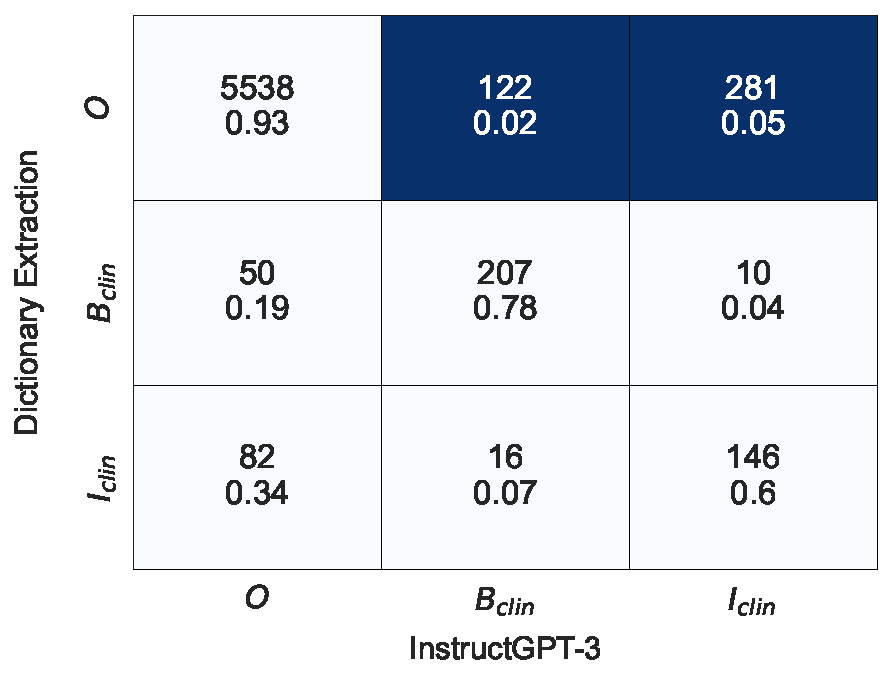
\includegraphics[height=2in]{figures/weak_supervision_healthnlp_2023/fr.layer2.validation_heatmap}
        \caption{Layer 2 validate}
        \vspace{4mm}
    \end{subfigure}
    \begin{subfigure}[t]{0.5\textwidth}
        \centering
        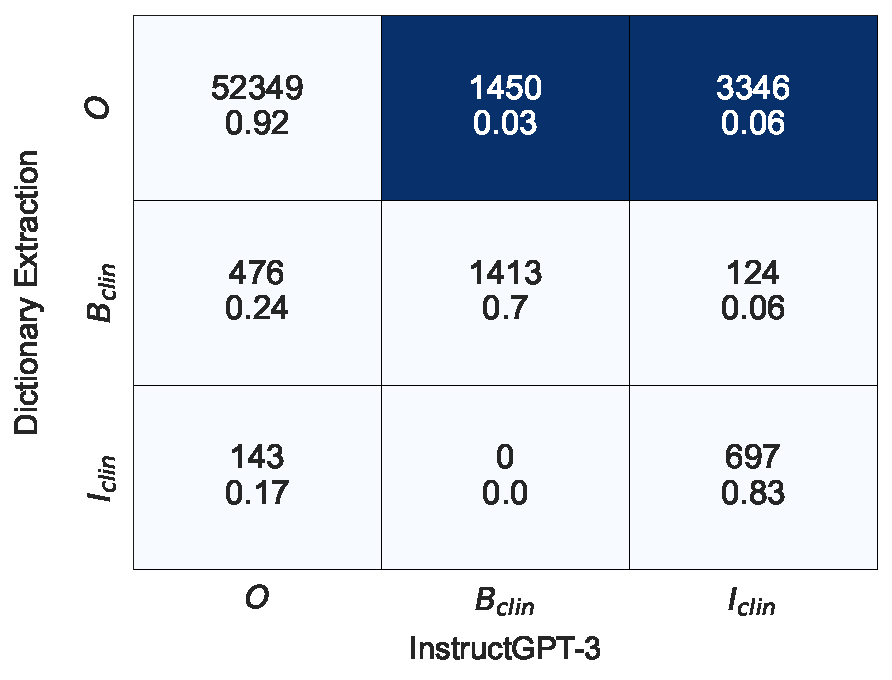
\includegraphics[height=2in]{figures/weak_supervision_healthnlp_2023/fr.layer2_heatmap}
        \caption{Layer 2}
    \end{subfigure}
    \caption{This figure represents the confusion matrices for the \textbf{layer~2} and the \textbf{layer~2~validate}. The matrices show the relationship between the dictionary annotations and via InstructGPT-3. For example, in the LayerValidate, the intersection of $B_{clin}$ (x-axis) to $O$ (y-axis) indicates that InstructGPT identified 122 tokens $O$ as $B_{clin}$ based on the dictionary extraction. The blue-coloured cells highlight the overflow of tokens annotated by InstructGPT-3 compared to the Dictionary Extraction annotation.}
    \label{fig:healthnlp_confuse}
\end{figure}

\paragraph{Knowledge Distillation Evaluation} We compare the distilled model (\textit{Instruct-Distilation}) and InstructGPT-3 on the \textbf{layer~1}. Both models have almost the same performance (Table \ref{tab:healthnlp_layer1}). Therefore, The distilled model has better precision, whereas InstructGPT performs better in recall.
\begin{table}
\centering
\large
\resizebox{0.7\textwidth}{!}{%
\begin{tabular}{@{}llll@{}}
\toprule
Models               & F1-Score           & Precision     & Recall             \\ \midrule
\distilInstruct & 0.74 $\pm$ 0.006 & \textbf{0.72} $\pm$ 0.01 & 0.78 $\pm$ 0.006 \\ \midrule
\instruct        & 0.74               & 0.70          & \textbf{0.81}               \\ \bottomrule
\end{tabular}%
}
\caption{
Comparison of InstructGPT-3 with a model distilled via weak supervision on the E3C \Ssilver, in terms of F1-score, Precision and Recall. Scores are calculated on the \Sgold.}
\label{tab:layer-1}
\end{table}


\paragraph{\textbf{Setting A}} If we compare the global F1-Score (Table \ref{tab:healthnlp_layer2}), the model trained with InstructGPT-3 supervision (\textit{Instruct-Distilation}) perform better than the model (\textit{Weak-Supervised Model}) trained 
with dictionary extraction supervision. 
In detail, the has a better F1-Score with $B_{clin}$ class, but the Recall and F1-score of $I_{clin}$ are relatively lower. 
The dictionary extraction tends to extract well one-word clinical terms, but this method does not cover multi-word terms. 
InstructGPT-3 has a better recall and recognizes multi-word clinical terms more easily. Still, this flexibility, balanced by the too-biased detection of false positive terms, lowered the precision score.
\begin{table}
\centering
\resizebox{0.40\textwidth}{!}{%
\begin{tabular}{@{}lll@{}}
\toprule
Annotations & \multicolumn{1}{l}{Dictionary Extraction} & InstructGPT-3 \\ \midrule
\multicolumn{1}{l}{F1-score}  & 0.69 $\pm$ 0.04 & \textbf{0.74} $\pm$ $6 e^{-3}$ \\ \midrule
\multicolumn{1}{l}{\bclin} &
  \begin{tabular}[c]{@{}l@{}}F: \textbf{0.76} $\pm$ 0.02\\ P: \textbf{0.83} $\pm$ $2e^{-3}$\\ R: 0.70 $\pm$ $4e^{-2}$\end{tabular} & 
  \begin{tabular}[c]{@{}l@{}}F: 0.73 $\pm$ $8e^{-3}$\\ P: 0.68 $\pm$ 0.02\\ R: \textbf{0.80} $\pm$ 0.01\end{tabular} \\ \midrule
\multicolumn{1}{l}{\iclin} &
  \begin{tabular}[c]{@{}@{}}F: 0.34 $\pm$ 0.10\\ P: \textbf{0.69} $\pm$ 0.01\\ R: 0.24 $\pm$ 0.08\end{tabular} &
  \begin{tabular}[c]{@{}@{}}F: \textbf{0.53} $\pm$ 0.01\\ P: 0.41 $\pm$ 0.01\\ R: \textbf{0.74} $\pm$ 0.01\end{tabular} \\ \bottomrule %
\end{tabular}%
}
\caption{F1-Score, Recall and Accuracy obtained using the \SettingA\space with the two different annotation sets. The scores of the F1-score line are the macro-F1-scores aggregated from the O, \bclin, \iclin.} 
\label{tab:layer-2}
\end{table}

\paragraph{\textbf{Setting B}} The amount of annotated tokens is relatively small compared to \textbf{layer~2} (Table \ref{tab:healthnlp_counts}). 
This hurts the result (Table \ref{tab:healthnlp_layer2validate}) of the \textit{Weak-Supervised Model} ($0.57$ with layer 2 validate vs $0.69$ with \textbf{layer~2}) in contrast to the \textit{Instruct-Distilation}, where performance is relatively equivalent. Still, the stability between the 5 folds is affected ($0.01$ with \textbf{layer~2~validate} vs $6e^{-3}$). The same fold stability issue is present for \textit{Weak-Supervised Model}, possibly due to the relatively small amounts of tokens on the train set.
\begin{table}
\centering
\resizebox{0.40\textwidth}{!}{%
\begin{tabular}{@{}lll@{}}
\toprule
Annotations & \multicolumn{1}{l}{Dictionary Extraction} & InstructGPT-3 \\ \midrule
 \multicolumn{1}{l}{F1-score} & 0.57 $\pm$ 0.02                                                & \textbf{0.74} $\pm$ 0.01                             \\ \midrule
 \multicolumn{1}{l}{\bclin} &
  \begin{tabular}[c]{@{}l@{}}F: 0.72 $\pm$ 0.03\\ P: \textbf{0.65} $\pm$ 0.07\\ R: 0.82 $\pm$ 0.04\end{tabular} &
  \begin{tabular}[c]{@{}l@{}}F: \textbf{0.74} $\pm$ 0.03\\ P: 0.64 $\pm$ 0.06\\ R: \textbf{0.87} $\pm$ 0.02\end{tabular} \\ \midrule
 \multicolumn{1}{l}{\iclin} &
  \begin{tabular}[c]{@{}l@{}}F: 0.02 $\pm$ 0.04\\ P: 0.33 $\pm$ 0.30\\ R: 0.01 $\pm$ 0.02\end{tabular} &
  \begin{tabular}[c]{@{}l@{}}F: \textbf{0.53} $\pm$ 0.01\\ P: \textbf{0.42} $\pm$ 0.03\\ R: \textbf{0.71} $\pm$ 0.03\end{tabular} \\ \bottomrule
\end{tabular}%
}
\caption{F1 score, Recall and Precision using E3C \layerTwo\space validate as the train set with both different annotations (dictionary extraction with manual correction and InstructGPT prediction),  the performance is computed on \layerOne.}
\label{tab:layer-2-validate}
\end{table}


\paragraph{\textbf{Setting C}} The results (Table \ref{tab:healthnlp_layer2blended}) shows slightly better performance for both models. We note that the \textit{Weak-Supervised Model} has a better recall for $I_{clin}$ than the \textit{Weak-Supervised Model} trained with only weak-supervision annotations ($0.24$ with \textbf{layer~2} vs. $0.35$ with \textbf{layer~2} mixture). The \textit{Instruct-Distilation} has better precision for $B_{clin}$ and $I_{clin}$ compared to \textit{Instruct-Distilation} trained with \textbf{layer~2}.   
In conclusion, mixing datasets with a low proportion of manual annotations reduces the tendency of each method to detect predictions of clinical terms that are smaller in terms of words (\textit{Weak-Supervised Model}) or encompass larger word sets (\textit{Instruct-Distilation}). 
\begin{table}
\centering
\large
\resizebox{0.40\textwidth}{!}{
\begin{tabular}{@{}lllll@{}}
\toprule
Annotations & \multicolumn{1}{l}{Dictionary Extraction} & InstructGPT-3\\ \midrule
F1-score  & 0.73 $\pm$ 0.01                                                 & \textbf{0.75} $\pm$ $5e^{-3}$                        \\ \midrule
\bclin &
  \begin{tabular}[c]{@{}@{}l@{}}F: \textbf{0.78} $\pm$ $7e^{-3}$\\ P: 0.84 $\pm$ $4e^{-3}$\\ R: \textbf{0.72} $\pm$ 0.01\end{tabular} &
  \begin{tabular}[c]{@{}l@{}}F: 0.77 $\pm$ $5e^{-3}$\\ P: \textbf{0.85} $\pm$ 0.01\\ R: 0.71 $\pm$ 0.01\end{tabular} \\ \midrule
\iclin &
  \begin{tabular}[c]{@{}l@{}}F: 0.46 $\pm$ 0.03\\ P: \textbf{0.66} $\pm$ 0.04\\ R: 0.35 $\pm$ 0.04\end{tabular} &
  \begin{tabular}[c]{@{}l@{}}F: \textbf{0.50} $\pm$ 0.01\\ P: 0.64 $\pm$ 0.02\\ R: \textbf{0.42} $\pm$ 0.02\end{tabular} \\ \bottomrule
\end{tabular}%
}
\caption{F1-score, Recall and Precision using E3C \layerTwo\space merged with \layerValidate\space (the layer where 10\% of the \layerTwo\space has been fixed manually) as the train set with both different annotations (dictionary extraction with manual correction and InstructGPT prediction), the performance is computed on \layerOne.}
\label{tab:layer-2-blend}
\end{table}

\paragraph{\textbf{Setting D}} The results indicate that using a ratio of $0.5$ between the annotation predicted by InstructGPT-3 and the annotation predicted by dictionary extraction allows improving the F1-Score by $0.03$ compared to the use of a dataset entirely annotated with the annotation predicted by InstructGPT-3 (i.e. when the ratio is 1). Moreover, incorporating a proportion of annotations predicted by InstructGPT-3 above $0.5$ allows for better stability between different folds. In conclusion, combining these two disparate annotation methods regarding recall and precision provides a good balance and increases the F1-Score.

\begin{figure}
    \centering
    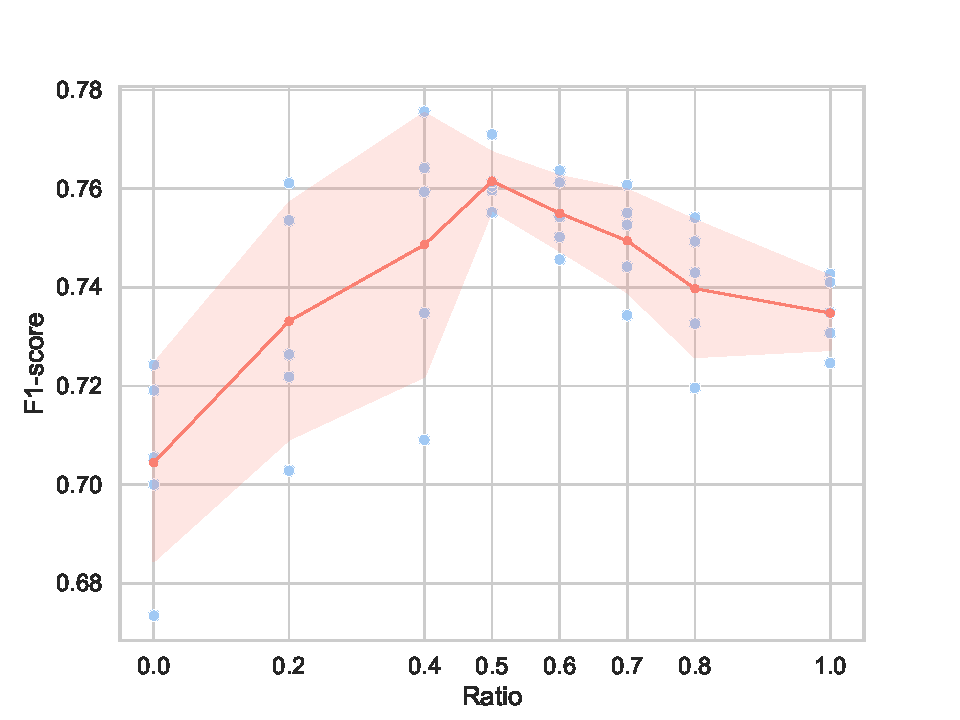
\includegraphics[width=\columnwidth]{figures/weak_supervision_healthnlp_2023/scatters.pdf}
    \caption{The figure represents a graph with the F1-score on the y-axis and the ratio of dictionary annotations and annotations via InstructGPT-3 on the x-axis as specified in the \textbf{Setting D} (Section \ref{sec:healthnlp_prot}). A ratio of 0 indicates the presence of only dictionary annotations, while a ratio of 1 corresponds to exclusively InstructGPT-3 annotations. Each blue dot represents a different experiment with a different data set. Each orange dot represents the mean of the experiments for a given ratio. The light orange filled part represents the standard deviation for a given ratio}.
    \label{fig:healthnlp_scatter}
\end{figure}

\begin{table}
    \centering
    \small
    \resizebox{0.40\textwidth}{!}{
        \begin{tabular}{@{}cccc@{}}%
\toprule%
Setting&F1{-}Score&Precision&Recall\\%
\midrule%
A&0.74 $\pm$ 0.01&0.69 $\pm$ 0.01&0.83 $\pm$ 0.01\\%
B&0.74 $\pm$ 0.02&0.69 $\pm$ 0.03&\textbf{0.84} $\pm$ 0.01\\%
C&0.75 $\pm$ 0.00&\textbf{0.82} $\pm$ 0.01&0.71 $\pm$ 0.01\\%
D&\textbf{0.76} $\pm$ 0.01&0.73 $\pm$ 0.02&0.81 $\pm$ 0.03\\\bottomrule%
%
\end{tabular}
    }
    \caption{This is the F1-score, Precision and the Recall for each settings in Section \ref{sec:healthnlp_prot}.}
    \label{tab:healthnlp_global}
\end{table}

\paragraph{Comparison of the different configurations} According to the results reported in Table \ref{tab:healthnlp_global}, Setting D is the one which obtained a slightly better F1-score ($0.76$). The mixture of dictionary annotations and InstructGPT-3 obtained with $r=0.5$ reduces the gap between the Recall ($0.81$) and Accuracy ($0.73$) scores. This allows us to assert that the two methods can be complementary: a combination of the two allows us to obtain a greater diversity of annotations than the use of only one of the two methods.

